\documentclass[a4paper, UKenglish, 11pt]{uiomaster}
\usepackage{lipsum}
\usepackage[subpreambles=true]{standalone}
\usepackage{graphicx}

\begin{document}

%TODO:
% Multocomparment models
% Fix explanation net sum is zero currents over membrane
% Fox V insead of phi
% Some figures to illustrate
% Point source approximation?

\chapter{Electroencephalograpy}
Neurons communicate with each other through the use of electical currents. When a neuron receives a signal, it generates an electrical current that propegates along the axon and causes the release of neurotransmitters that diffuse across the gap between the sending and the recieving neuron. If the neurotransmitters are accepted by the receptors on the recieving neuron, a new electrical signal, also known as synaptic input will be generated. This transmission of signals between neurons at specialized junctions are called synaptic inputs. The process of electrical communaication between neurons creates electromagnetic fields that can be measured using electroencephalography (EEG).

Electroencephalography (EEG) is a non-invasive technique that has been used for almost a century to study the electrical potentials in the human brain. It has remained one of the most important methods for investigating the brain's activity, with significant applications in both neuroscientific and clinical research \cite{ilmoniemi2019brain}.

% Maybe this should appear in introduction to neurosience
An EEG signal is believed to originate from large numbers of synaptic inputs to populations of geometrically aligned pyramidal neurons \cite{nunez2006electric}.The signal can be understood as a signature of neural activities that are generated from synaptic inputs to cells in the cortex. Synaptic inputs on its side are electrical or chemical signals that are being transmitted from one neuron to another, causing changes in the membrane potential of the neurons. In other words, neurons are specialized to pass signals, and synapses are the structures that make this transmission possible.

One of the primary uses of EEG is to investigate cognitive processes, diagnose diseases, and estimate functional connectivity. To measure the electrical activity in the brain, small metal disks called electrodes are placed on the scalp, which detect the electrical charges that result from the activity of brain cells. This technique can help identify abnormalities in specific areas of the brain, indicating potential signs of disease. Thus, EEG can be used to evaluate various brain disorders, including lesions, Alzheimer's disease, epilepsy, and brain tumors. An illustration of the typical EEG measurement setup is depicted in Figure \ref{fig:EEG}.

\begin{figure}[!htb]
    \centering
    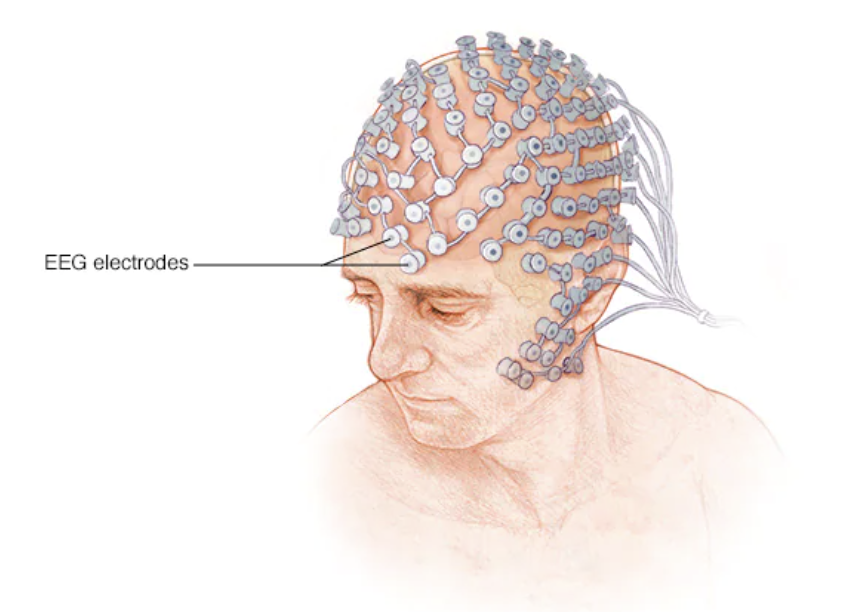
\includegraphics[width=\linewidth]{figures/EEG_fig.png}
    \caption{Illustration of the EEG method.}
    \label{fig:EEG}
\end{figure}


Source localization is a fundamental aspect of EEG signal analysis, with the ultimate aim of accurately identifying the location of neural current sources from EEG data. However, this is a challenging problem due to the inherent ill-posed nature of the inverse problem in electrostatics. This means that there is no unique solution, making it a difficult task to solve. Before digging deeper into the inverse problem, we will first look at how to simulate electrical brain activity and the corresponding EEG signal as it would have been measured by electrodes on the scalp. This method is better known as forward modeling.

\section{Forward modeling of EEG signals}
To better understand the complexities of the inverse problem and the nuances of source localization in EEG, it is helpful to gain a deeper comprehensionin of forward modeling, involving the simulation of electrical activity of the brain as it would be measured by electrodes on the scalp.

As explained in chapter 1, neural activity generates electric currents in the brain, which in turn create electromagnetic fields. In order to calculate extracellular electric potentials, one can envision the head as a 3D volume conduction, and combine Maxwell's equations with the current conservation law. We then obtain the Poisson equation for computing extracellular potentials:

\begin{equation}
  \nabla \cdot \textbf{J} = \nabla \cdot \left(\sigma \nabla \phi \right)
\label{eq:Poisson}
\end{equation}

where \textbf{J} is the electric current density in extracellular space, $\sigma$ is the extracellular conductivity and $\phi$ is the extracellular electric potential \cite{naess2021biophysically}. For simple, symetric head models, the Poisson equation can naturally be solved analytically. However, as for the New York Head which is a complex model that we will be utialize in this thesis, we will be using the numerical method known as Finite Element Method (FEM) when solve the quation.


To accurately calculate the extracellular potential(s), $\phi$, a well-established two-step forward-modeling approach is used. In the first step, a multicompartmental model is utialized, which takes into account the intricate details of neuron morphologies to determine the transmembrane currents, $I_n$. In the second step, equation \ref{eq:Poisson} is solved, under the assumptions that the extracellular medium acts as a volume conductor with the following properties:

\begin{itemize}
    \item infinitely large
    \item linear
    \item ohmic
    \item isptropic
    \item homogeneous
    \item frequency-independent
\end{itemize}

The origin of extracellur potentials is spatially distributed membrane currents, entering and escaping the extracellular medium. These currents can be understood as current sources and sinks, and give the extracellular potential, $\phi$ at the electrode location $\textbf{r}$:

\begin{equation}
  \phi(\textbf{r}) = \frac{1}{4\pi\sigma}\sum^{N}_{n=1}\frac{I_n}{|\textbf{r}-\textbf{r}_n|}
\label{eq:extracellular_potential}
\end{equation}

where $\textbf{r}_n$ is the location of the tranmembrane current $I_n$, $N$ is the number fof transmembrane currents and $\sigma$ is the extracellular conductivity \cite{naess2021biophysically}.

\section{Multicompartmental modeling}
The potential over the membrane, $V_m$, in long neurons with multi-branched dendrites varies depending on whether the potential is measured in the soma or at the tip of a sital denrite \cite{naess2021biophysically}. Multicompartmental (MC) models are models that account for this spatial variabilty in $V_m$. In such models, the neural morphology commonly is represented as isopotential cylindrical compartmens, with lengths and diameters derived from reconstructed morphologies, connected with resistors \cite{sterratt2011principles}. Single values of $V_m$ can then be computed for each individual compartment, as depiced in Figure \ref{fig:MC_models}.

%TODO:
% Fix figure text and sources
\begin{figure}[!htb]
    \centering
    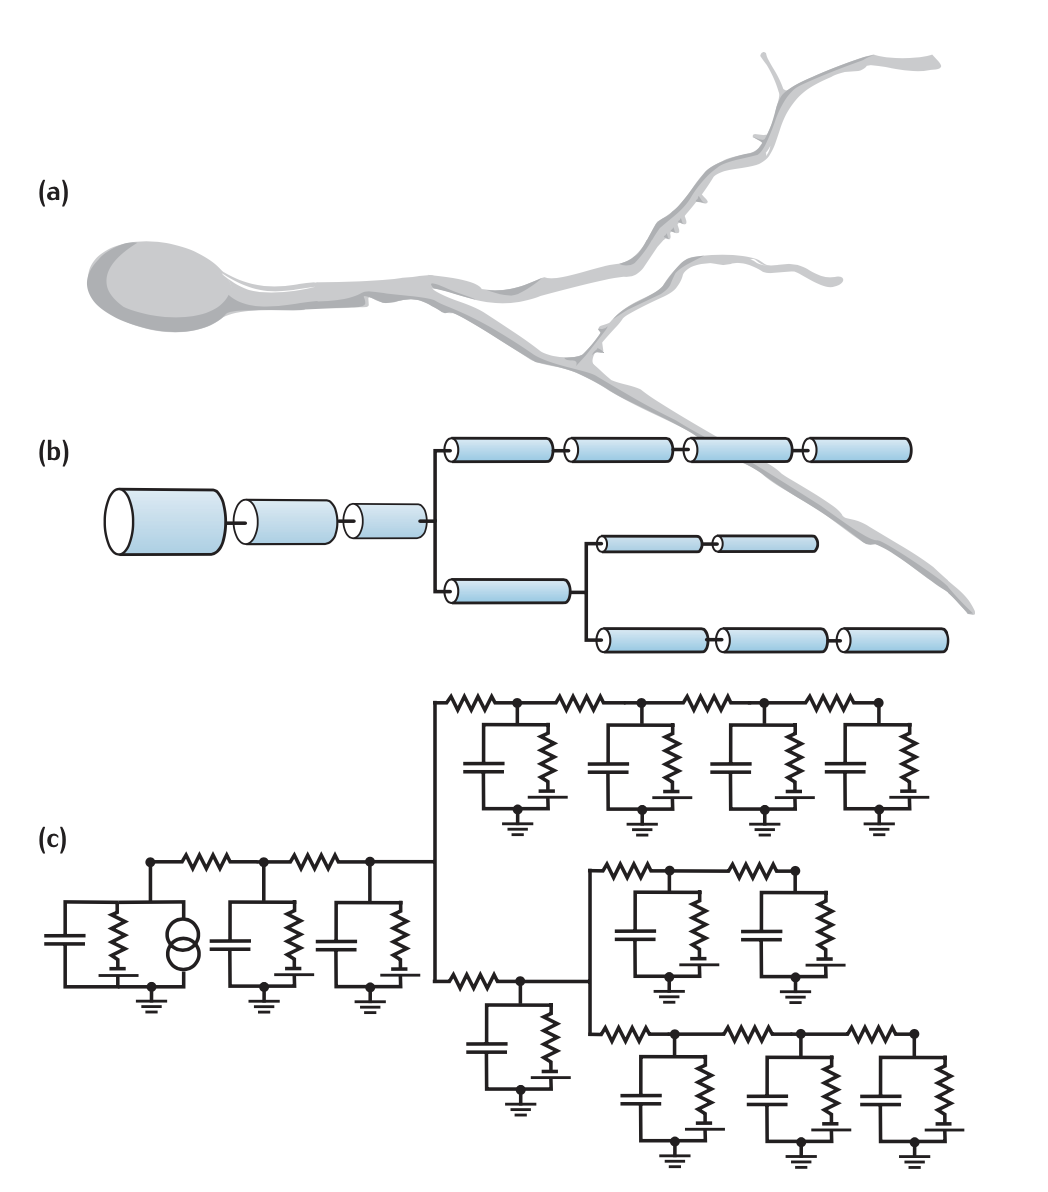
\includegraphics[width=\linewidth]{figures/MC_models.png}
    \caption{A diagram of the development of a multi-compartmental model.
(a) The cell morphology is represented by (b) a set of connected cylinders. An electrical circuit consisting of (c) interconnected RC circuits is then built from the geometrical properties of the cylinders, together with the membrane properties of the cell.}
    \label{fig:MC_models}
\end{figure}

The fundamental equation for MC models is given as:
\begin{equation}
  c_m\frac{dV_{m,n}}{dt} = - i_{L,n} - \sum_w i_{w,n} - \frac{I_{\text{syn},n}}{\pi dL} + \frac{I_{\text{ext},n}}{\pi dL} \frac{d}{4r_a}\left( \frac{V_{m,n+1} - V_{m,n}}{L^2} - \frac{V_{m,n} - V_{m,n-1}}{L^2} \right )
\label{eq:MC}
\end{equation}

where ....

This equation (\ref{eq:MC}) assumes that a compartment $n$ has two neighbors - one at $n - 1$ and the second at $n - 2$. However, when considering the endpoint compartments, this clearly will not be true. A commonly used boundry condition, is the sealed-end condition, where no axial currents leave at the cable endpoints. With other words this means that $I_{0,1} = 0$ in one end of the cable, and $I_{N,N+1} = 0$ in the other end. For the cable endpoints, we are then left with the following expressions:

\begin{equation}
  c_m\frac{dV_{m,1}}{dt} = - i_{L,1} - \sum_w i_{w,1} - \frac{I_{\text{syn},1}}{\pi dL} + \frac{I_{\text{ext},1}}{\pi dL} \frac{d}{4r_a}\left( \frac{V_{m,2} - V_{m,1}}{L^2} \right )
\label{eq:MC_end1}
\end{equation}

and

\begin{equation}
  c_m\frac{dV_{m,N}}{dt} = - i_{L,N} - \sum_w i_{w,N} - \frac{I_{\text{syn},N}}{\pi dL} + \frac{I_{\text{ext},n}}{\pi dL} \frac{d}{4r_a}\left( \frac{V_{m,N} - V_{m,N-1}}{L^2} \right )
\label{eq:MC_end2}
\end{equation}

%TODO
% Some equation for the

\section{Volume conductors}
As mentioned above, we can use volume conductor (VC) theory to predict the resulting extracellular potential $V_e$ at any given point in space, given that the distribution of neuronal membrane currents is known.

% What should I include here?

\section{Current Dipole Approximation}

EEG signals are generated from synaptic inputs to cells in the cortex. Synaptic inputs are electrical (or chemical) signals that are being transmitted from one neuron to another, causing changes in the membrane potential of the neurons. In other words, neurons are specialized to pass signals, and synapses are the structures that make this transmission possible.

When calculating extracellur potentials, $V_e$, at large distances from the underlying current sources, one is typically benefitted with using the current-dipole approximation. This approximation is justifided by the fact that a neuron's contribution to $V_e$ becomes increasingly dipolar with increasingly distance and is commonly utialized when simulating EEG signals.

We know that electrical charges can create current multipoles, depending on coordinates and symmetry of the charge distribution \cite{wiki:multipoles}. Analogous, the combination of current sinks and sources set up such charge multipoles.
When the distance $R$ from the center of the volume to the recording point is larger that the distance from the volume center to the most peripheral source, multipole expansion can be used \cite{jackson1999classical}. When utializing the multipole expansion theorem equations \ref{eq:extracellular_potential} can be expressed as follows:

\begin{equation}
  \phi(R) = \frac{C_{\text{monopole}}}{R} + \frac{C_{\text{dipole}}}{R^2} + \frac{C_{\text{quadrupole}}}{R^3} + \frac{C_{\text{octopole}}}{R^4} + ... .
\label{eq:extracellular_potential}
\end{equation}

where the numerators represents the contributions to the extracellular potential. The terms denoted $C_\text{monopole}$, $C_\text{dipole}$ and $C_\text{quadrupole}$ represents contributions to the extracellulat potential, $V_e$, and can in general be extremely complicated as they depend on the relationship between radial coordinates and symmetry of the current source and measurement electrode. However, multiple expansions are often beneficial as usually only the first few terms are needed in order to provide an accurate approximation of the original funtion. This also turns out to be true in our case, as the quadrupole, octople and higher-order contributions to $V_e$ decay more rapidly with distance $R$ than the dipole contibution. Assuming that we are sufficiently far away from the source distribution, all terms above the dipole contribution vanish. As for the monopole contribution, we know that since ...... the net sum of currents over a neuronal membrane is always zero. This means that also the monopole term vanishes, and the expression for the extracellular potential, $V_e$ is approximated by the dipole contribution alone:

\begin{equation}
\phi(\textbf{r}) \approx \frac{C_{\text{dipole}}}{R^2} = \frac{1}{4\pi\sigma}\frac{|\textbf{p}| cos \theta}{|\textbf{r}-\textbf{r}_p|^2}.
\label{eq:extracellular_potential_approximation}
\end{equation}

where we have substituded for $C_\text{dipole}$ in terms of other properties. $\textbf{p}$ denotes the current dipoile moment in a medium with conductivity $\sigma$. $R = |\textbf{R}| = |\textbf{r} - \textbf{r}_p|$ is the distance between the current dipole moment at $\textbf{r}_p$ and the electrode lokation $\textbf{r}$. Finally $\theta$ represents the angle between $\textbf{p}$ and $\textbf{R}$. This equation is known as the dipole approximation and is a precise approximation for calculating extracellular potential, given that $R$ is much larger than the dipole length $d=|\textbf{d}|$, like in the case of EEG \cite{naess2021biophysically}.

Having that a current dipole moment $\textbf{p}$ can be predicted from an axial current $I$ inside a neuron and the distance vector $\textbf{d}$ traveled by the axial current we get the following expression: $\textbf{p} = I\textbf{d}$. Generalising this equation, we get that the relationship between the current dipole moment, $\textbf{p}$ and a \emph{set} of neural current sources can be expressed as follows:

\begin{equation}
\textbf{p} = \Sigma^N_{n=1}I_n\textbf{r}_n
\label{eq:extracellular_potential_approximation}
\end{equation}

In figure \ref{fig:dipole_pattern} we have provided a simulation of the extracellular potential generated by a neuron in response to a single synaptic input, where the spatial distribution of membrane current was explicitly taken into consideration. Based on the figure, it is apparent that the distribution of electric charge in the extracellular potential of the neurons surroundings  exhibits distinct dipole patterns when observed from a greater distance.

\begin{figure}
    \centering
    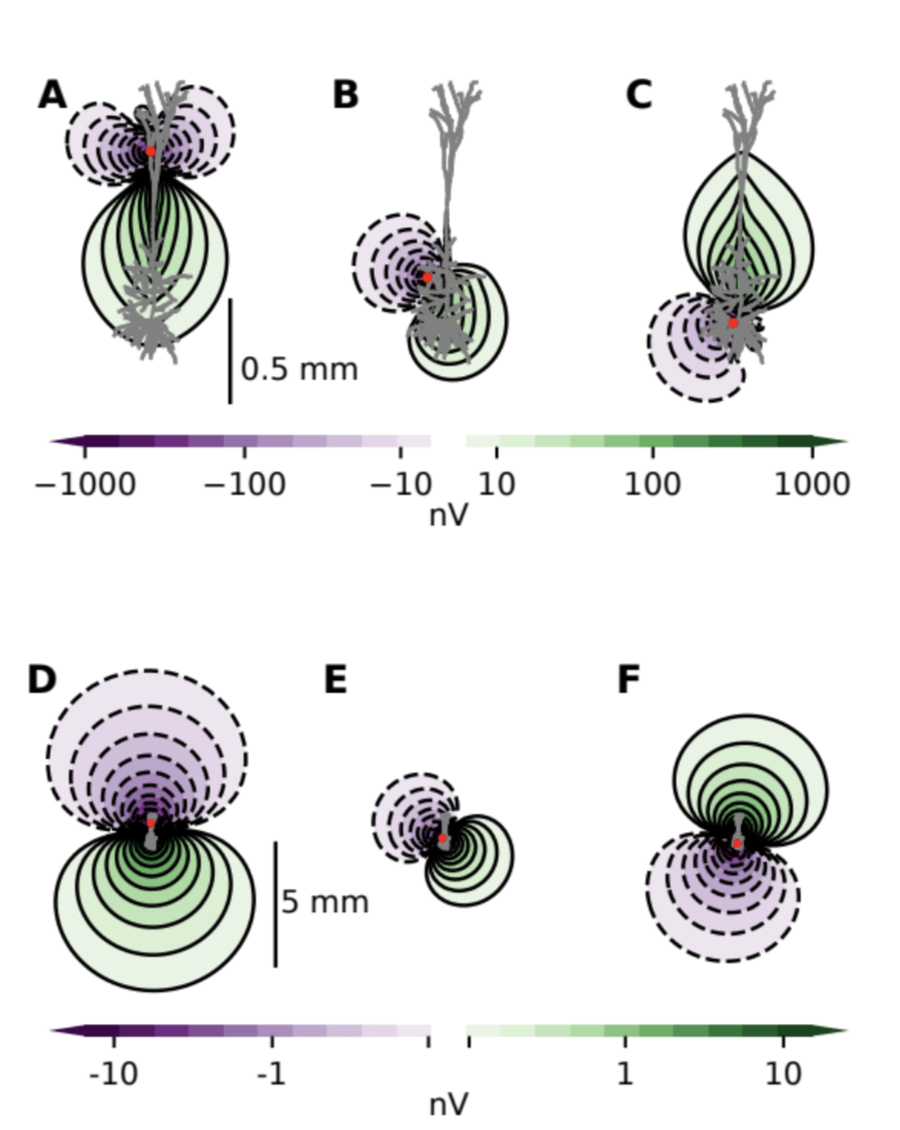
\includegraphics[width=\linewidth]{figures/dipole_pattern.png}
    \caption{Source and explanation.}
    \label{fig:dipole_pattern}
\end{figure}


\section{Head Models}
The analytical formula presented in Equation \ref{eq:extracellular_potential_approximation} was dereived based on the assumption of a constant tissue conductivity, denoted as $\sigma$. However, because the EEG signals is measured outside the head, it is affected by the different conductivities og the brain, verebrospinal fluid (CSF), skull and scalp. Depending on problem, it may be important to keep in mind that EEG signals, in general, are significantly affected by biophysically details of the head. For instance, the conductivity of the cerebrosipinal fluid exhibits a conductivity of approximately 1.7 S/m, while the conductivity of the scull and scalp is approximately 0.01 S/m and 0.5 S/m, respectively. These conductivity variations highlight the need for more comprehensive and realistic models of the head, known as head models, which take into account such conductivity variations. In addition to acount for the variations in conductivity across different regions of the head, head models also takes into account that the EEG signal from a neuronal population will depend on whether the population is located in a \emph{sulcus} or a \emph{gyrus} \cite{naess2021biophysically}. Said with other words, by integrating biophysical details into models, a deeper understanding emerges regarding the impact of various tissues on the distribution of extracellular potential, which in turn, can lead to improvements in the accuracy of EEG signal analysis.


\subsection{The New York Head}
A central problem for EEG is to relate scalp data to brain \emph{current sources} (Electric Fields of the Brain: The Neurophysics of EEG)....

Especially important for electrode locations outside of the brain, such as EEG, is the knowledge about how the electrical potentials will be affected by the geometries and conductivites of the various parts of the head \cite{naess2021biophysically}. A model that takes these detailes into account is the New York Head Model. The model is based on anatomical and electrical characteristics of 152 adult human brains and is solved for 231 electrode locations.

The New York Head Model is a computer model of the human head used to simulate the electrical activity of the brain. It was created by the Electrical Geodesics Incorporated (EGI) in 2004, and is based on the anatomical and electrical characteristics of the head of a typical adult human. The model consists of a three-dimensional (3D) representation of the head and brain, with detailed information on the geometry and electrical properties of the different tissues and structures within the head. The model includes the scalp, skull, cerebrospinal fluid, gray matter, and white matter. The electrical properties of each of these tissues, such as conductivity and permittivity, are also included in the model.
% Need sources and to be rewritten

The model was developed to be used for, and improve the accuracy of EEG source localization \cite{huang2016new}. To generate predictions of the EEG signals recorded from different scalp locations in response to a given set of source currents, the New York head model uses the lead field matrix (SOURCE), which is a mathematical representation of the relationship between the electrical activity in the brain and the electrical potentials recorded on the scalp.

\begin{figure}
  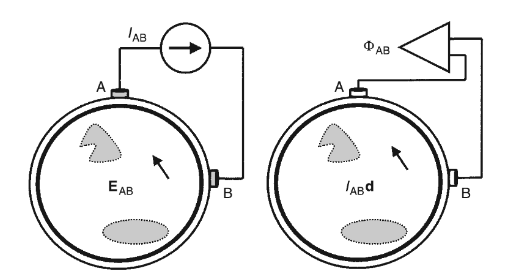
\includegraphics[width=\linewidth]{figures/lead_fields.png}
  \caption{A caption here is needed.}
  \label{fig:lead_field}
\end{figure}

The lead field matrix is constructed by taking advantage of the reciprocity theorem that states that knowledge of the current density through a volume conducter caused by an injection of current between two stimulating electrodes completely specifies how those same recording electrodes pick up potentials caused by dipole sources in the volume conducter. If one suppose that a pair of stimulating electrodes is placed at locations A and B on the scalp as provided in figure \ref{fig:lead_field}, an external current source will cause current to flow from electrode B through the brain, and all the way to electrode A. However, due to the geometry, inhomogeneity, and ansisotropy of the head, the current density will vary with location. The amount of current that pass through the brain depends, to a great extent, on the location of the electordes. In general, the brain currents will decrease with decreasing distance between electrodes. Thus, for a fixed pair of electrodes, the lead field vectors can be calculated as a function of position throughout a volume conducter. At each location, the orientation of the lead field vector $L_{AB}$ is the orientation of the dipole source that produces the largest potential difference between the electrodes. The lead field matrix, $\boldsymbol{L}$ is given as:

\begin{equation}
L = \frac{E}{I},
\label{eq:R2}
\end{equation}

where $I$ is the injected current at the electode locations and $E$ is the resulting electric field in the brain \cite{naess2021biophysically}. Moreover, the precise link between a current dipole moment $p$ in the brain and the resulting EEG signals $\Phi$ is then related to the lead field matrix as follows:

\begin{equation}
\Phi_{AB} = L_{AB} \cdot p,
\label{eq:EEG_signal}
\end{equation}

Here, an injected current $I$ of 1 mA gives an electric potential $E$ in V/m, meaning that a current dipole moment $\textbf{p}$ in the unit of mAm gives EEG signals in the unit of V.

%(Do I understand this? Note: Can write much more about this. page 288.)

The New York Head model has been incorporated in the Python module LFPy, which provides classes for calculation of extracellular potentials from multicomparment neuron models. These tools will be utialized in this thesis. For more information read: \url{https://lfpy.readthedocs.io/en/latest/readme.html#summary}

%\section{Current Dipoles Approximation}
%EEG signals arise from cortical neural activity and are typically described in terms of current dipoles.

%An optimal model of EEG signals would have consisted of multiple dipole moments. However, as such a model is complicated and computationally expensive, we will in this project only introduce one single dipole approximation $\textbf{p}(t)$ for each multicompartmental neuron simulation. In this context, by  multicompartmental modelling we refer to the widely used models within neuroscience, which acurately manufactures electical properties of single neurons. The sigle-dipole approximation might sound like a substantial simplification of the real biophysical properties, nevertheless it actually turns out to give a realistic modelling of EEG signals, when handling the single dipole moment, as an abnormality in the brain. We will be thinking of the abnormality as an epileptic seizures or a tumor in the brain, which among normal activity in the brain would have stuck out. The single-dipole approximation is implemented by summing up the multiple current dipole moments,
%\begin{equation}
%    \textbf{p}(t) = \sum_{k=1}^M \textbf{p}_k(t) = \sum_{k=1}^M I_k^{\text{axial}}(t)\textbf{d}_k,
%\end{equation}
%where $I^{\text{axial}}$ is the current flowing along the neurite with the distance vector $\textbf{d}_k$ and $M$ denotes the number of axial currents. The data set we will be using in this project will consist of measures of different EEG signals at a given time from 1000 patients. This means that we for each patient pick a random location (at $t=0$) for the single current dipole.

%\section{The New York Head Model}
The signals received from EEG are known to originate from cortical neural activity, which are often described by using current dipoles. It is therefor reasonable to implement current dipoles in the brain for when generating a biophysical modeling of EEG signals. The brain model used in this thesis is called the New York Head model, and is based on high-resolution anatomical MRI-data from 152 adult heads. The model utilizes the software tool LFPy, which is a Python module for calculation of extracellular potentials from multicompartment neuron models. This model takes into account that electrical potentials are effected by the geometries and conductivities of various parts of the head.

The cortex matrix consists of 74382 points, which refer to the number of possible positions of the dipole moment in the cortex. When generating our data set, we will for each sample randomly pick the position of the dipole moment, such that one sample corresponds to one patient. In our head model we are considering 231 electrodes uniformly distributed across the cortex, meaning that each EEG sample will consist of this many signals for each time step. However, we are not interested in the time evolution of the signals as this does not affect nor say anything about the position of the dipole moment, and we therefor simply pick out the EEG signals for when $t$ = 0 (note that the choice of time step could have been randomly picked). Our final design matrix will then consist of 1000 rows, corresponding to each patient, and 231 columns also refereed to as features, representing the signal of each electrode. The final output we are trying to predict is then the one dimensional vector with length 1000, where each element consists of the x-, y- and z- position of the dipole moment. An example of how the input EEG signals may look like is given in appendix A, where we also have marked the dipole moment with a yellow star.






%Imagining a small part of the cortex, all of these cells will have dendrites pointing upwards in the same direction (lets say the z-direction). Due to rotational symmetry around the z-axis, the contributions in the x- and y-direction will cancel. This is illustrated in Figure \ref{fig:EP}. What we see is that the extracellular potential is configured in all sorts of weird ways (A-C) when there is only one synaptic input, while the extracellular potential reminds more of a dipole when we have multiple synaptic inputs (D-F). We can therefore argue that the total contribution to the extracellular potential can be modelled as a dipole in the z -direction for the case where we have multiple synaptic inputs. Hence, for each dipole moment in our simulations, we assume multiple synaptic inputs, and make sure to rotate the positions of the dipoles such that it is orientated along the depth of the cortex.

%\begin{figure}
%    \centering
%    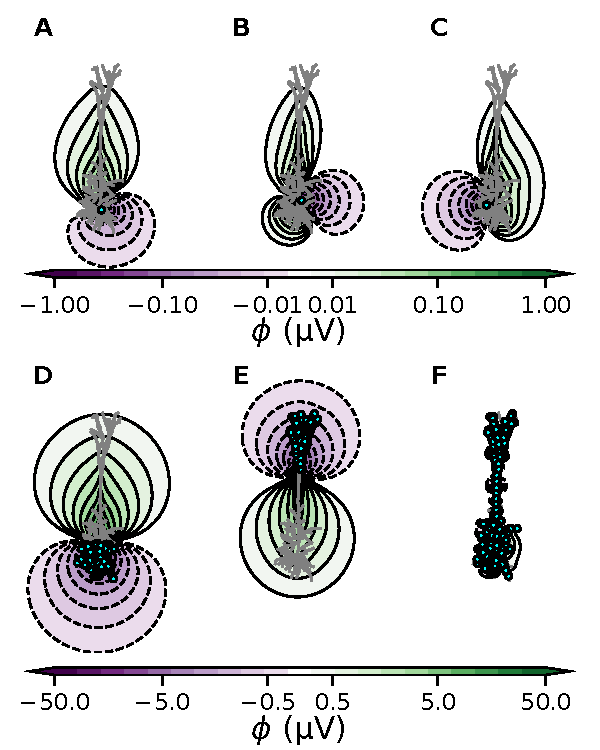
\includegraphics[width=\linewidth]{figures/fig_chosen_dipoles.pdf}
%    \caption{Extracellular potential from lonely synaptic input (A-C) and extracellular potential from multiple synaptic inputs (D-F).}
%    \label{fig:EP}
%\end{figure}


\section{The Inverse Problem and Source Localization}

% To solve the inverse EEG problem, various algorithms and methods have been developed, such as Minimum Norm Estimates (MNE), Low Resolution Electromagnetic Tomography (LORETA), and Dynamic Imaging of Coherent Sources (DICS). MACHINE LEARNIG....

% The inverse EEG problem is the problem of determining the sources of electrical activity within the brain that give rise to the measured EEG signal. The EEG signal is a recording of the electrical activity of the brain, which is measured at the surface of the scalp. However, the electrical activity that gives rise to the EEG signal is generated by a large number of sources within the brain, and it is not possible to determine the location or number of these sources just by looking at the EEG signal alone. Therefore, the inverse EEG problem is the problem of determining the sources of the EEG signal based on the measurement of the signal itself.

% To solve the inverse EEG problem, various algorithms and methods have been developed, such as Minimum Norm Estimates (MNE), Low Resolution Electromagnetic Tomography (LORETA), and Dynamic Imaging of Coherent Sources (DICS).

% However, the problem remains very challenging, as the EEG signal measured at the scalp is the result of a complex and unknown combination of sources, the brain anatomy itself and the volume conductor contribute to the complexity of the problem.

% As of now, there is not yet a definitive solution for the Inverse EEG problem and the area is still active research topic.

\end{document}